\section{Concept}
In this section a concept of a mobile \enquote{\gls{see}} version will be presented. 
Therefore, a prototype will be created to point out the features that a mobile version of \enquote{\gls{see}} requires.

Prototypes are a common way to express the needs of a system. 
It is a low-cost way of planning an implementation, that can highlight challenges regarding constraints of a system early on.

Even though a prototype will never be able to show every aspect and need of a complex system, it should still help to answering questions like: 
How should the system feel? How should it be implemented and what are the key features? \cite{houde1997prototypes} 

\enquote{\gls{see}} is meant to be used by multiple platforms such as desktop devices, mobile devices and virtual reality devices.
Each device has different interaction constrains. 
While a desktop user will control the player with mouse and keyboard a mobile user will interact with virtual joysticks on a touchscreen.
Selecting nodes of a \enquote{\gls{city}} will be done by clicking it with a mouse on desktop devices, while a mobile device will require a touch input.

\subsection{Interface}

\begin{figure}[htb]
    \centering
    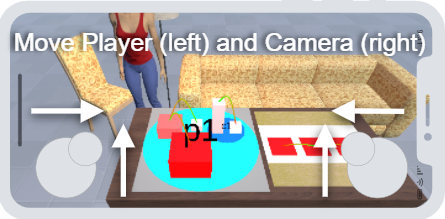
\includegraphics[width=1\textwidth]{Concept/img/joystick.png}
    \caption{Joysticks for moving in \enquote{\gls{see}}}\label{fig:joystick}
\end{figure}

\begin{figure}[htb]
    \centering
    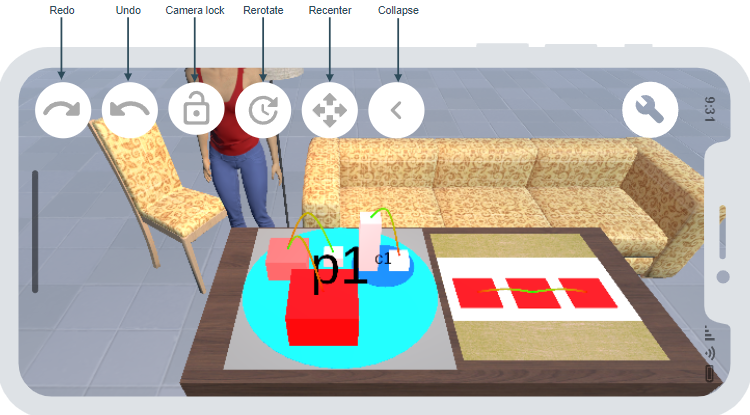
\includegraphics[width=1\textwidth]{Concept/img/quickbar.png}
    \caption{Quickbar for various interactions in \enquote{\gls{see}}}\label{fig:quickbar}
\end{figure}

\begin{figure}[htb]
    \centering
    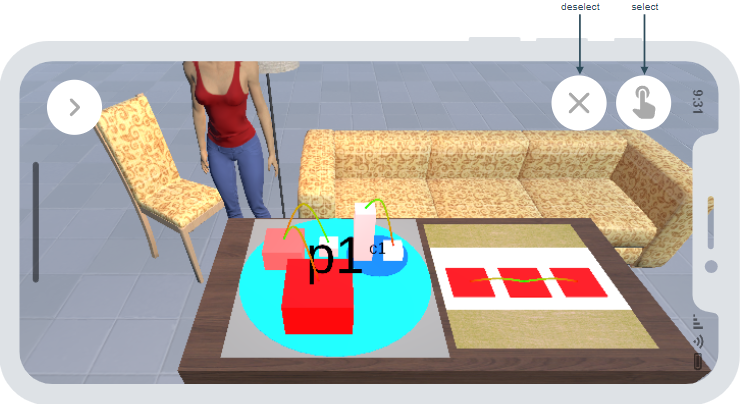
\includegraphics[width=1\textwidth]{Concept/img/menu1.png}
    \caption{Selection mode in \enquote{\gls{see}}}\label{fig:select}
\end{figure}

\begin{figure}[htb]
    \centering
    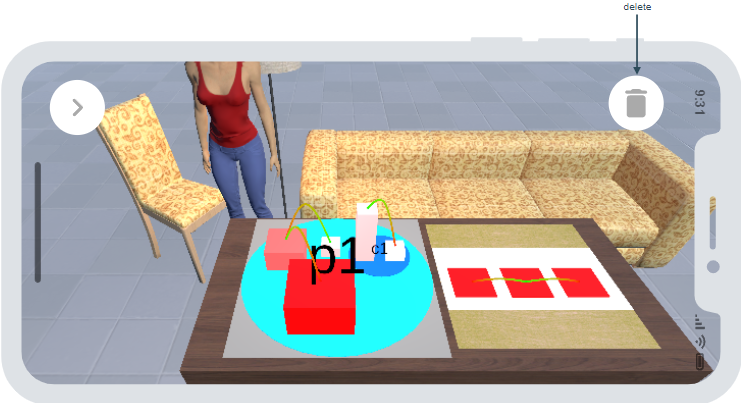
\includegraphics[width=1\textwidth]{Concept/img/menu2.png}
    \caption{Delete mode in \enquote{\gls{see}}}\label{fig:delete}
\end{figure}

\begin{figure}[htb]
    \centering
    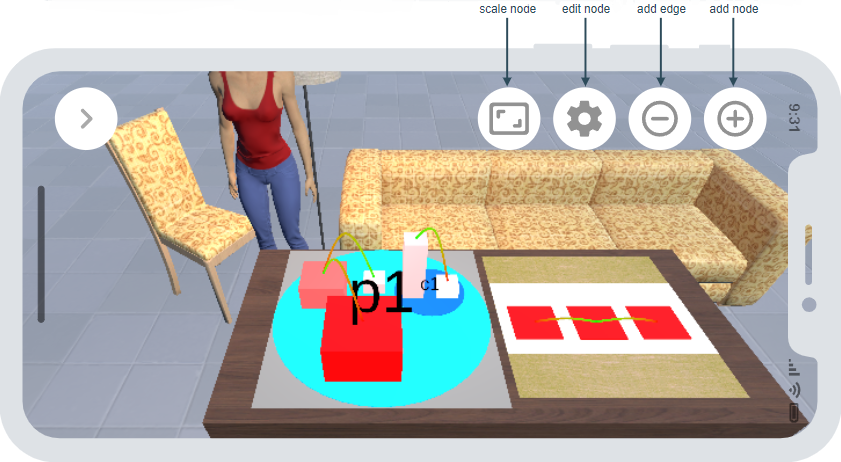
\includegraphics[width=1\textwidth]{Concept/img/menu3.png}
    \caption{Node interactions in \enquote{\gls{see}}}\label{fig:nodes}
\end{figure}

\begin{figure}[htb]
    \centering
    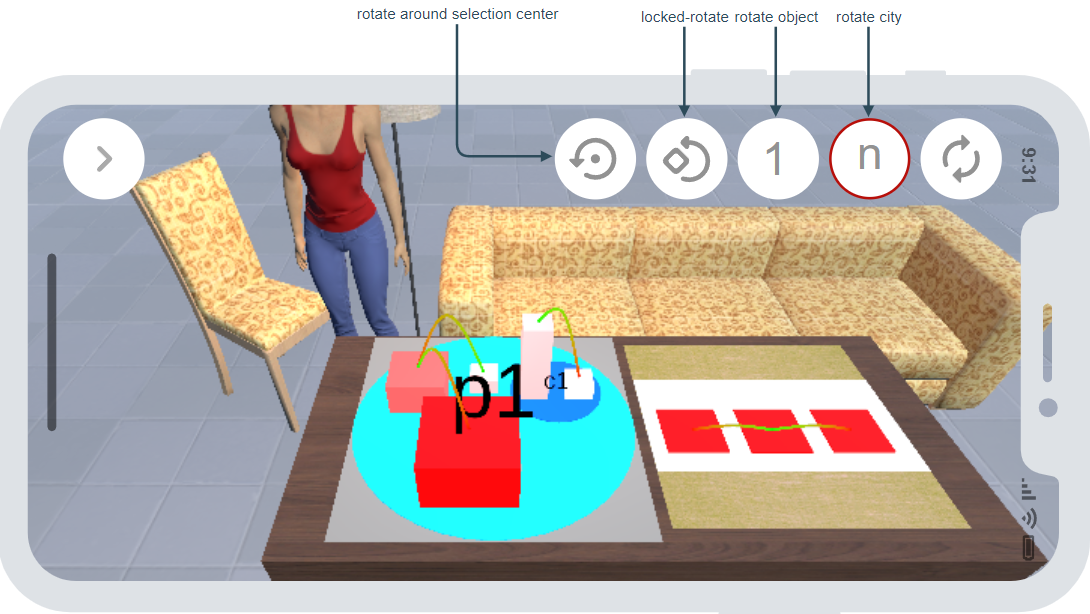
\includegraphics[width=1\textwidth]{Concept/img/menu4.png}
    \caption{Rotation mode in \enquote{\gls{see}}}\label{fig:rotate}
\end{figure}

\begin{figure}[htb]
    \centering
    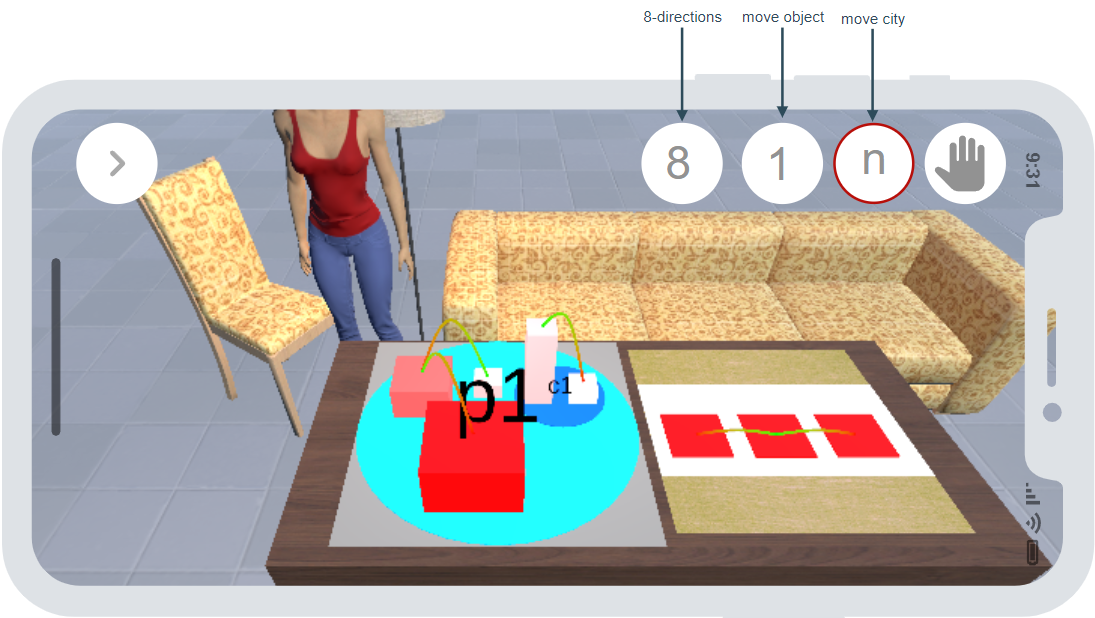
\includegraphics[width=1\textwidth]{Concept/img/menu5.png}
    \caption{Movement mode in \enquote{\gls{see}}}\label{fig:move}
\end{figure}

\subsection{Interaction}
...
\subsection{Requirements}
In the following a list of requirements will be given, which will specify in detail what the implementation of a mobile version has to take care of.
The list will be referred to multiple times in the upcoming realization part in chapter \ref{section:implementation}.
Requirements are essential for the planning phase as they give a good fundamental structure for the developer to rely on. \cite{Robertson2012,Stevens2005}